\documentclass{beamer}
%\documentclass[notes=only]{beamer}

\usepackage[utf8]{inputenc}
 
\usetheme{Dresden}

\title[Visualisation and GBL for DSA teaching] %optional
{Exploring Visualisation and Game-Based Learning tools for teaching Data Structures and Algorithms}
  
\author{Edward Zhang \and Simon Su}
 
\institute[UoA] % (optional)
{
  Department of ECSE\\
  The University of Auckland
}
 
\date[May 2019] % (optional)
{Literature Review Seminar}

\begin{document}
\frame{\titlepage}
\section{Introduction}
\subsection{Research Intent}
\begin{frame}
  \frametitle{Research Intent and Summary}
  What we found...
  \begin{itemize}
    \item Relatively few Game-Based Learning tools for DSA
    \item Game-Based Learning (GBL) tools and Algorithm Visualisations (AVs) are proven tools to improve learning outcomes
    \item Even fewer learning tools contain both GBL and AVs
  \end{itemize}
  \pause
  We propose further research into a tool that offers GBL within a game world, alongside AVs that take advantage of the analogies and interactivity afforded by said game world.
\end{frame}
\subsection{Teaching DSA}
\begin{frame}
  \frametitle{Why DSA?}
  Data Structures and Algorithms are an essential topic in Computer Science-related fields, and form the foundation of many higher-level concepts in CS.
  \note{...therefore, it's v. important for students to develop a solid understand of DSA earlier in their studies. This importance is the motivation for focusing our research on developing tools for teaching DSA}
\end{frame}
\begin{frame}
  \frametitle{DSA Curriculum}
  The ACM CS2013 provides guidelines on subjects that should be taught in an undergrad CS course. Algorithms \& Complexity is identified as a core Knowledge Area and within that the knowledge unit of Fundamental Data Structures and Algorithms.
  \pause
  \begin{block}{Our Implementation}
  We will focus on teaching Fundamental DSA for the purposes of the tool we intend to develop.
  \end{block}
\end{frame}
\begin{frame}
  \frametitle{Fundamental DSA in ACM CS2013}
  \begin{itemize}
    \item Simple Numeric Algorithms
    \item Sequential and Binary Search
    \item Quadractic and $\Omega(n\log(n))$ sorting algorithms
    \item Hash tables and collisions
    \item Binary search trees
    \item Graphs and common graph algorithms
    \item Heaps
    \item Pattern matching/string algorithms
  \end{itemize}
  \note{These are the fundamental DSA as defined by CS2013. While it is beyond the scope of this project to implement all of these in our tool, we will focus on a subset of these DSAs and take into the learning outcomes mentioned in CS2013 when working on the content to implement in our tool}
\end{frame}
\begin{frame}
  \frametitle{DSA Learning Outcomes in CS2013}
  We will target some of the learning outcomes outlined in CS2013...
  \begin{enumerate}
    \item Implement basic numerical algorithms.
    \item Be able to implement common quadratic and $\Omega(n\log(n))$ sorting algorithms.
    \item Discuss the runtime and memory efficiency of principal algorithms for sorting, searching, and hashing.
    \item Demonstrate the ability to evaluate algorithms, to select from a range of possible options, to provide justification for that selection, and to implement the algorithm in a particular context. 
  \end{enumerate}
  \note{Ideally, our tool would help students achieve these 4 learning outcomes, although the last one may be hard to achieve within a game, further work and research needed.}
\end{frame}
\section{Algorithm Visualisation}
\begin{frame}
  \frametitle{What is Algorithm Visualisation?}
  \begin{block}{A note on Simon}
    Simon's section goes here, but unfortunately he's decided to produce it in Keynote.
  \end{block}
\end{frame}
\section{Game-based Learning}
\begin{frame}
  \frametitle{What is Game-based Learning?}
  Recently, educational games have started to be employed as a tool to assist classroom learning. But why?
  \pause
  \begin{itemize}
    \item Educational games are argued to appeal to students of all ages
    \item Students can learn at their own pace and re-attempt problems
    \item Understanding is enhanced through the use of immersive environments
    \item Some games designed solely for entertainment have been shown to be highly educational
  \end{itemize}
  \pause
  There also exists a special relationship between digital educational games and computer science education, as programming is the foundation of said games.
\end{frame}
\begin{frame}
  \frametitle{7 Billion Humans}
  A wildly popular puzzle game (rated ``Very Positive'' on Steam) from developers of ``World of Goo'' where plays program workers (humans) to perform tasks to solve the puzzle. Uses a block-based assembly-like language for programming. Of interest is that this wasn't designed as a educational game. Unfortunately no studies on the educational nature of this game.
\end{frame}
\begin{frame}
  \begin{center}
    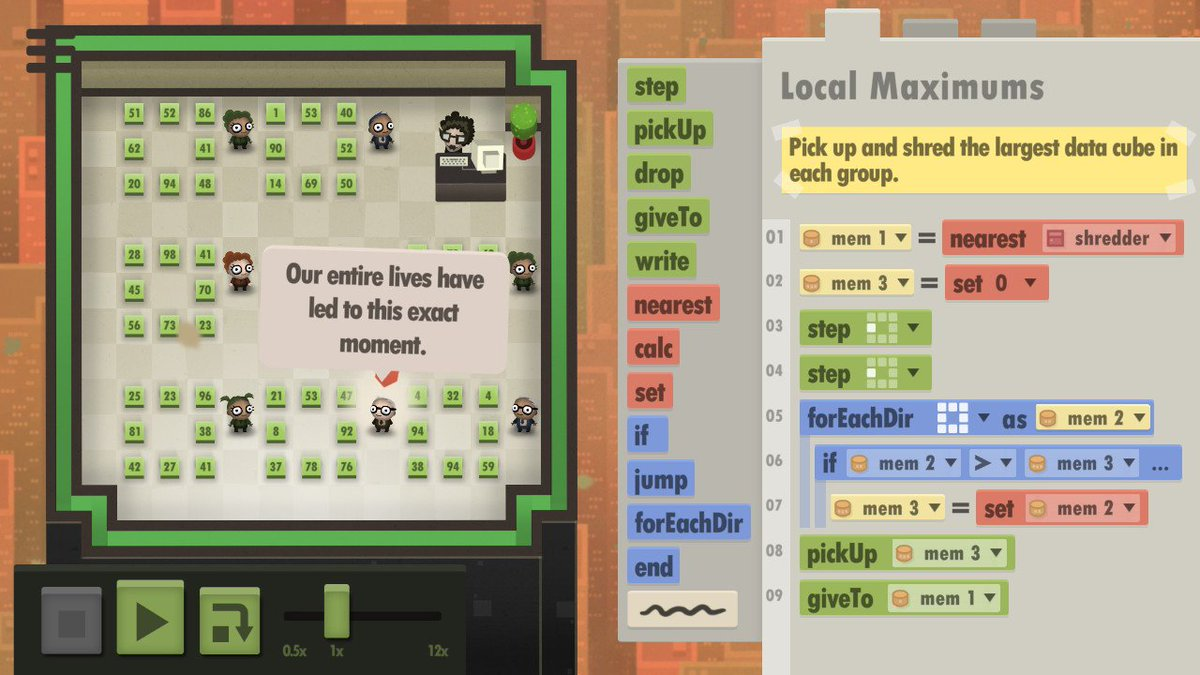
\includegraphics[width=\textwidth,height=\textheight,keepaspectratio]{7bnhumans.jpg}
  \end{center}
\end{frame}
\begin{frame}
  \frametitle{Lightbot}
  A more traditional educational game, where you navigate a robot (lightbot) around the map. Programming uses a much simpler block \& icon based language. Unlike 7BH, lightbot was designed with teaching basic programming in mind.
  \note{Lightbot has actually been evaluated for it's educational use by various papers. More on this later.}
\end{frame}
\begin{frame}
  \begin{center}
    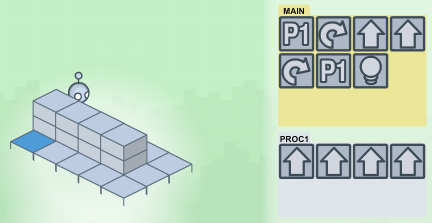
\includegraphics[width=\textwidth,height=\textheight,keepaspectratio]{lbot.png}
  \end{center}
\end{frame}
\subsection{Evaluating GBL}
\begin{frame}
  \frametitle{A evaluation of GBL with boardgames}
  The paper ''Design and Large-scale Evaluation of Educational Games for Teaching Sorting Algorithms`` focuses on evaluating DSA games with students, in order to determine the effectiveness of (their) GBL.\\
  \note{They test both board and digital games...}
  \pause
  Games tested involved board and digital games for teaching Heapsort and Quicksort.
\end{frame}
\begin{frame}
  \begin{center}
    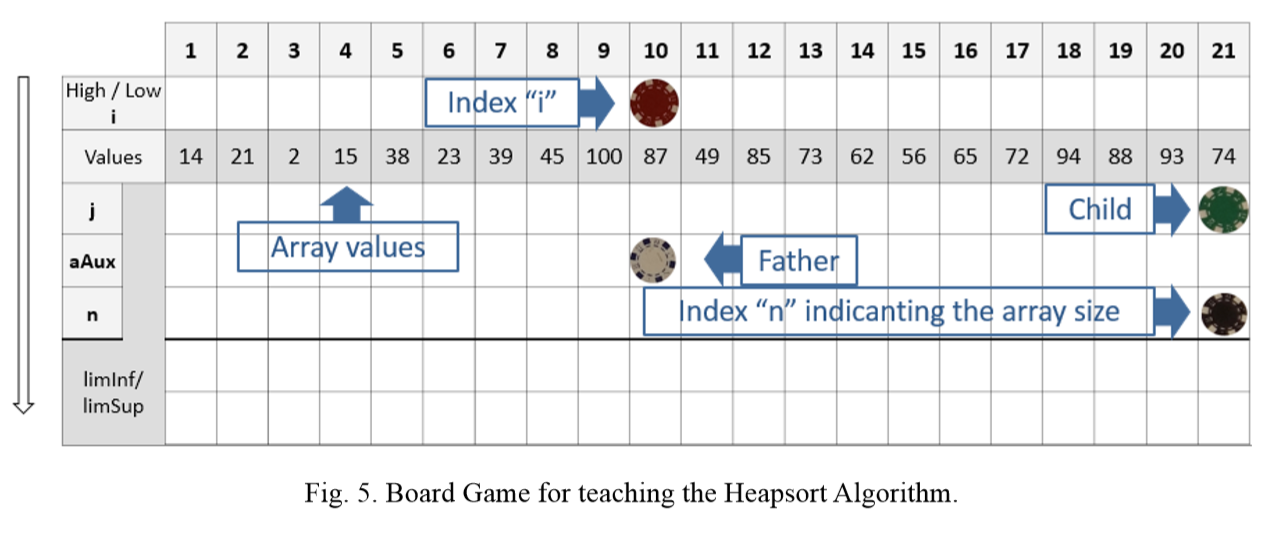
\includegraphics[width=\textwidth,height=\textheight,keepaspectratio]{boardgame.png}
  \end{center}
\end{frame}
\begin{frame}
  \frametitle{Evaluation}
  Authors evaluated the games across $\geq 300$ students, across different year levels and courses. Students played the game and evaluated using a questionnaire based on MEEGA (Model for the Evaluation of Educational GAmes).
  \note{talk about MEEGA}
\end{frame}
\begin{frame}
  \frametitle{Analysis Questions}
  The authors used the evaluation to answer these analysis questions\dots
  \begin{enumerate}
    \item Do the games motivate Students?
    \item Do the games provide a positive user experience?
    \item Do the games contribute to learning?
    \item What are the differences in the quality of the (three games tested) in relation to the above?
  \end{enumerate}
\end{frame}
\begin{frame}
  \frametitle{Evaluation evaluation}
  \begin{itemize}
    \item No pre-test measurement
    \item Self-assessment only
    \item Common evaluation model (MEEGA)
  \end{itemize}
\end{frame}
\begin{frame}
  \frametitle{PlayIt: Game Based Learning Approach for Teaching Programming Concepts}
  Study at Massey University into the effectiveness of GBL for programming, using the game LightBot.
\end{frame}
\begin{frame}
  \frametitle{Evaluation Design}
  \begin{itemize}
    \item Participants divided into three cohorts
    \item One played LightBot before attending classes
    \item One played LightBot after attending classes
    \item One did not use LightBot
  \end{itemize}
  Students filled out feedback immediately after survey and also at the end of study. Open ended questions and likert scale data. Student's pass rate was also analysed.
\end{frame}
\begin{frame}
  \frametitle{Evaluation evaluation}
  \begin{itemize}
    \item No common evaluation model
    \item No pre-test measurement
    \item Academic performance analysed, but sample size too small
  \end{itemize}
\end{frame}
\end{document}